\documentclass{article}

% Chinese Support using xeCJK
% \usepackage{xeCJK}
% \setCJKmainfont{SimSun}

% Chinese Support using CTeX
% \usepackage{ctex}

% Math Support
\usepackage{amsmath}
\usepackage{amsfonts}
\usepackage{amssymb}
\usepackage{wasysym}

% Graphics Support
\usepackage{graphicx}
\usepackage{float}

% Reduced page margin
\usepackage{geometry}
\geometry{a4paper,scale=0.8}

\usepackage{caption}
\usepackage{subcaption}

% d and e should be math operators
\newcommand*{\dif}{\mathop{}\!\mathrm{d}}
\newcommand*{\md}{\mathop{}\!\mathrm{d}}
\newcommand*{\me}{\mathrm{e}}

% No indent for each paragraph
\usepackage{parskip}
\setlength{\parindent}{0cm}

% Bold style for Greek letters
\usepackage{bm}
\let\Oldmathbf\mathbf
\renewcommand{\mathbf}[1]{\boldsymbol{\Oldmathbf{#1}}}

% More space for dfrac in cell
\usepackage{cellspace}
\setlength{\cellspacetoplimit}{5pt}
\setlength{\cellspacebottomlimit}{5pt}

% SI units
\newcommand{\si}[1]{\  \mathrm{#1}}

% Multi-line author information
\usepackage{authblk}
\author{Xiping Hu}
\affil{https://hxp.plus/}

\title{Homework for Chapter 11}

\begin{document}

\maketitle

\begin{figure}[H]
  \centering
  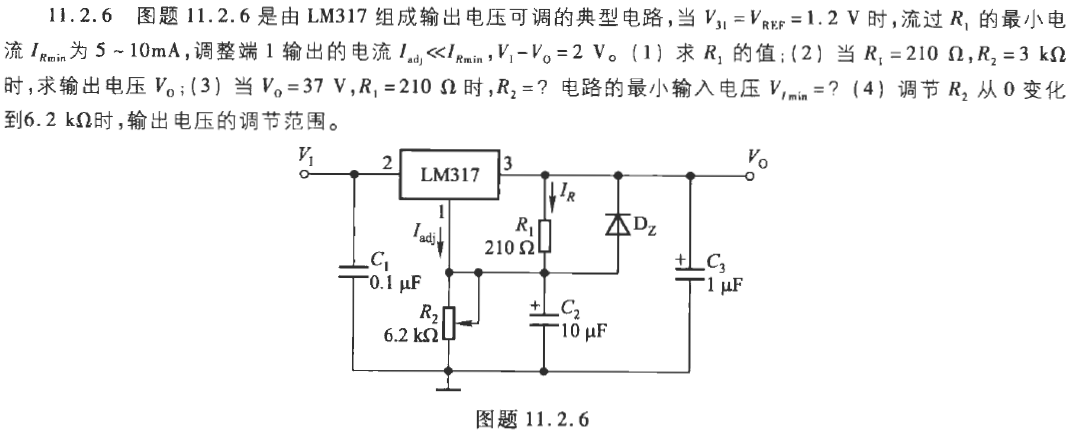
\includegraphics[width=\linewidth]{figures/Problem1126}
\end{figure}

\section{Problem 1}

\begin{equation*}
  \begin{aligned}
    R_1 = \dfrac{V_{REF}}{I_{R1min}} = 240 \rightarrow 120 \si{\Omega} 
  \end{aligned}
\end{equation*}

\section{Problem 2}

\begin{equation*}
  \begin{aligned}
    V_O = V_{REF} \left( 1 + \dfrac{R_2}{R_1}  \right) \approx 18.3 \si{V}
  \end{aligned}
\end{equation*}

\section{Problem 3}

\begin{equation*}
  \begin{aligned}
    37 = 1.2 \left( 1 + \dfrac{R_2}{210} \right) \Rightarrow R_2 \approx 6.3 \si{k\Omega}
  \end{aligned}
\end{equation*}

\section{Problem 4}

\begin{equation*}
  \begin{aligned}
    V_o = 1.2 \times \left( 1 + \dfrac{0}{210}  \right) \rightarrow 1.2 \times \left( 1 + \dfrac{6200}{210}  \right) = 1.2 \rightarrow 36.6 \si{V}
  \end{aligned}
\end{equation*}

\end{document}